%\documentclass{beamer}
\documentclass[handout]{beamer}

\usepackage[utf8]{inputenc}

\usetheme[bullet=circle,
          titleline=true,
          pageofpages=of,
          alternativetitlepage=true]{Torino}

\usepackage{color}

\usepackage{ragged2e}
\usepackage{hyphenat}

\usepackage{amsmath}
\usepackage{amsfonts}
\usepackage{amsthm}

%\usepackage{sympytex}
\usepackage{pythonhighlight}

\definecolor{MyGreen}{rgb}{0.40,0.80,0.20}

\title{SymPy --- a library for symbolic mathematics \linebreak in pure Python}
\author{Ondřej Čertík \texttt{<ondrej@certik.cz>}}
\institute[PWR]{University of Nevada, Reno\linebreak SymPy Development Team}
\date{August 19, 2009}

\newenvironment{jblock}[1]{
    \begin{block}{#1}\justifying\nohyphens
}{
    \end{block}
}

\begin{document}

\setbeamercovered{transparent}

\frame{\titlepage}

\begin{frame}[fragile]
    \frametitle{The Biggest Little City in the World}
    \begin{center}
        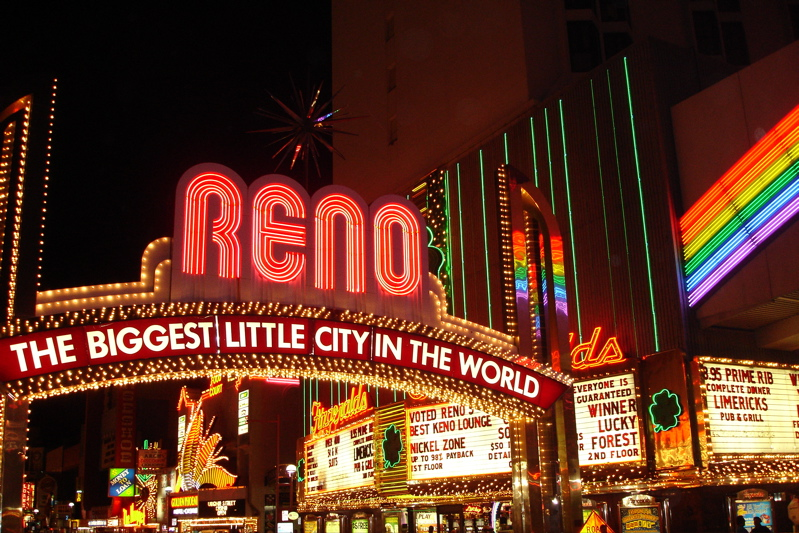
\includegraphics[width=4in]{images/Renoarch.jpg}
    \end{center}
\end{frame}

\begin{frame}[fragile]
    \frametitle{Reno}
    \begin{itemize}
        \item Till late 1950s, the gambling capital of the US
        \item Bars, clubs, easy marriage, easy divorce
        \item Best cross-country skiing in the US
        \item Awesome countryside, Lake Tahoe, MTB paradise
    \end{itemize}
    \begin{center}
        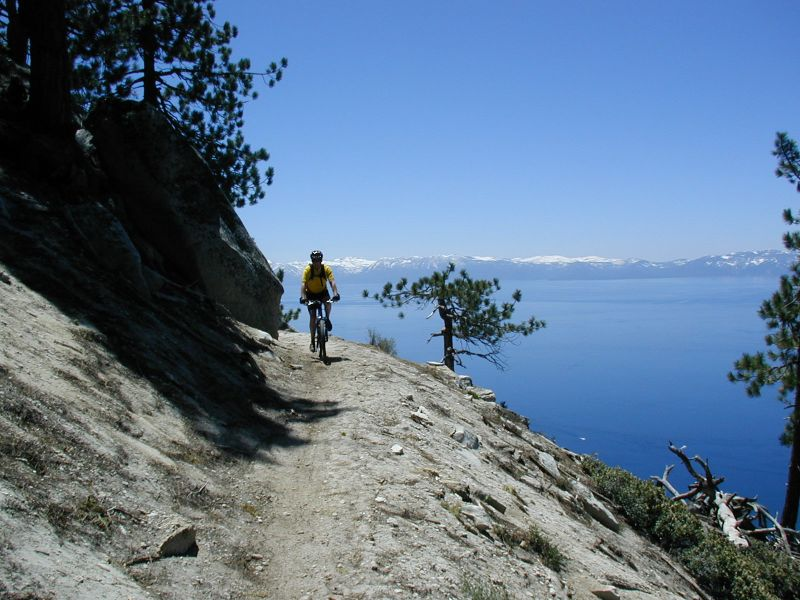
\includegraphics[width=2in]{images/tahoe1.jpg}
        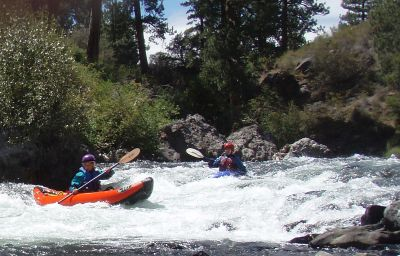
\includegraphics[width=2in]{images/truckee1.jpg}
    \end{center}
\end{frame}

\begin{frame}[fragile]
    \frametitle{What is SymPy?}

    \begin{itemize}
        \item A pure Python library for symbolic mathematics
        %\item A \structure<2>{pure} \structure<3>{Python} \structure<4>{library}
        %      for \structure<5>{symbolic} \structure<6>{mathematics}
    \end{itemize}

    \onslide<2->
    \begin{python}
  >>> from sympy import *
  >>> x = Symbol('x')

  >>> limit(sin(pi*x)/x, x, 0)
  pi

  >>> integrate(x + sinh(x), x)
  (1/2)*x**2 + cosh(x)

  >>> diff(_, x)
  x + sinh(x)
    \end{python}
\end{frame}

\begin{frame}[fragile]
    \frametitle{Advantages of being pure Python}
    \begin{itemize}
        \item jython (sympy can be used in java applications)
        \item 1565 tests in 139 files on 21584 lines (pypy, jython, unladen swallow)
        \item some efforts to get it run on top of CLPython (on lisp)
        \item google app engine
        \item iphone
        \item easy to deploy on windows
    \end{itemize}
\end{frame}


\begin{frame}[fragile]
    \frametitle{Capabilities}
    \framesubtitle{What SymPy can do}

    \begin{columns}
        \begin{column}[l]{0.5\textwidth}
            \begin{itemize}
                \item core functionality
                    \begin{itemize}
                        \item differentiation, truncated series
                        \item pattern matching, substitutions
                        \item non--commutative algebras
                        \item assumptions engine, logic
                    \end{itemize}
                \item symbolic \ldots
                    \begin{itemize}
                        \item integration, summation
                        \item limits
                    \end{itemize}
                \item polynomial algebra
                    \begin{itemize}
                        \item Gröbner bases computation
                        \item multivariate factorization
                    \end{itemize}
                \item matrix algebra
            \end{itemize}
        \end{column}
        \begin{column}[r]{0.5\textwidth}
            \begin{itemize}
                \item equations solvers
                    \begin{itemize}
                        \item algebraic, transcendental
                        \item recurrence, differential
                    \end{itemize}
                \item systems solvers
                    \begin{itemize}
                        \item linear, polynomial
                    \end{itemize}
                \item pretty--printing
                    \begin{itemize}
                        \item Unicode, ASCII
                        \item LaTeX, MathML
                    \end{itemize}
                \item 2D \& 3D plotting
                \item \structure{\ldots}
            \end{itemize}
        \end{column}
    \end{columns}
\end{frame}

\begin{frame}[fragile]
    \frametitle{ASCII pretty--printing}

    \begin{center}
        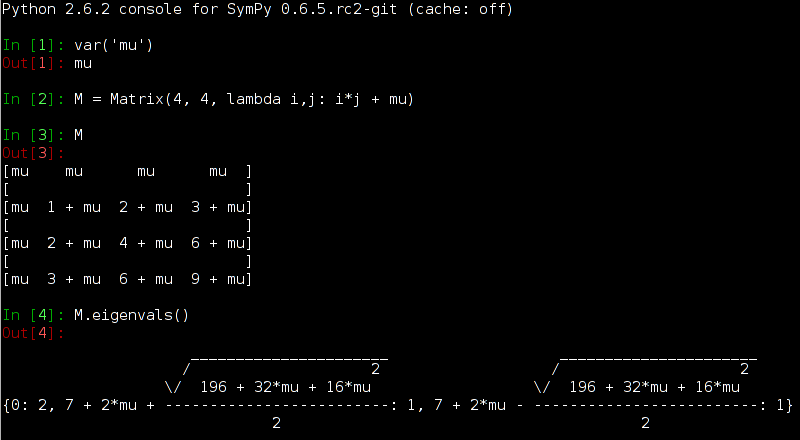
\includegraphics[scale=0.65]{images/sympy-ascii.png}
    \end{center}
\end{frame}

\begin{frame}[fragile]
    \frametitle{Unicode pretty--printing}

    \begin{center}
        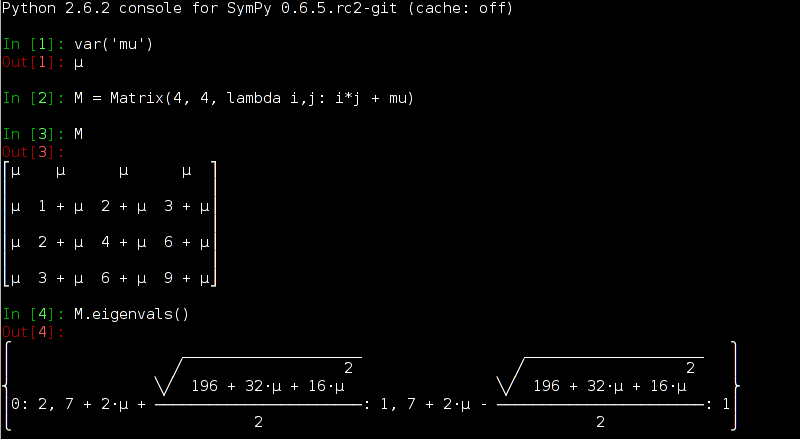
\includegraphics[scale=0.65]{images/sympy-unicode.png}
    \end{center}
\end{frame}


\begin{frame}[fragile]
    \frametitle{List of SymPy's modules (1)}

    \begin{description}
        \item[concrete] symbolic products and summations
        \item[core] Basic, Add, Mul, Pow, Function, \structure{\ldots}
        \item[functions] elementary and special functions
        \item[galgebra] geometric algebra
        \item[geometry] geometric entities
        \item[integrals] symbolic integrator
        \item[interactive] for setting up pretty--printing
        \item[logic] new assumptions engine, boolean functions
        \item[matrices] Matrix class, orthogonalization etc.
        \item[mpmath] fast arbitrary precision numerical math
    \end{description}
\end{frame}

\begin{frame}[fragile]
    \frametitle{List of SymPy's modules (2)}

    \begin{description}
        \item[ntheory] number theoretical functions
        \item[parsing] Mathematica and Maxima parsers
        \item[physics] physical units, Pauli matrices
        \item[plotting] 2D and 3D plots using pyglet
        \item[polys] polynomial algebra, factorization
        \item[printing] pretty-printing, code generation
        \item[series] compute limits and tructated series
        \item[simplify] rewrite expresions in other forms
        \item[solvers] algebraic, recurrence, differential
        \item[statistics] standard probability distributions
        \item[utilities] test framework, compatibility stuff
    \end{description}
\end{frame}

\end{document}

